\section{powerlaw distributed inputs}
This distribution has mostly small values, but occasionally it also generates bigger values.
The lower the parameter the higher the values get and also the amount of big values increases.
For a parameter of $\beta=2.75$ and a maximum value of 10,000 the distribution looks like in Figure~\ref{fig:powerDistExample1}.
All values are rather small and less than 100, also half of the values are one.
So this input seems rather easy for $\beta=2.75$.

\begin{figure}[h]
      \caption{Distribution of a random powerlaw input with $\beta=2.75$}
      \centering
      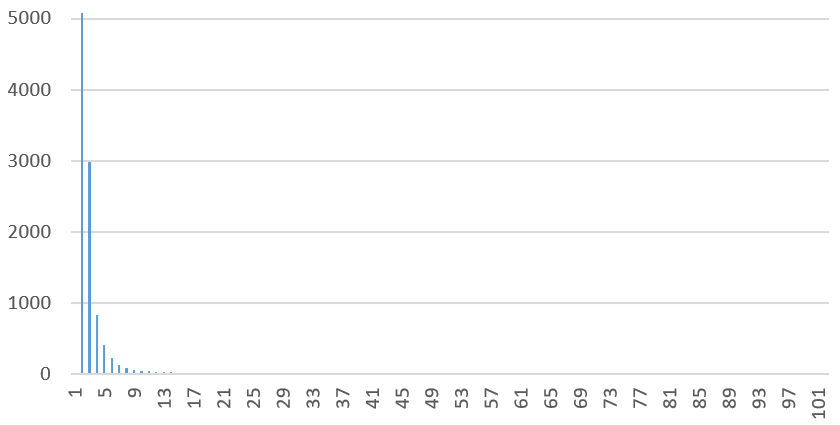
\includegraphics[width=0.7\textwidth]{figures/images/numberGenerator/powerlaw_-2_75.png}\label{fig:powerDistExample1}
\end{figure}

For a value of $\beta=1.25$ the distribution looks a bit different.
There are less small values close to one and instead also big values even over 1000.
Figure~\ref{fig:powerDistExample2} is cropped to get a more clear view for the smaller values.
The higher values mostly occurred 0 to 2 times.
The highest value 9948 occurred only once.
Researching inputs like this should be more interesting which is why for the experiment $\beta=1.25$ was chosen.
To give a better view on this type of input there is also a table $\beta=2.75$ at the evaluation of the (1+1) EA.\
The results for the other algorithms were mostly the same, but these are not shown here for better readability.

\begin{figure}[h]
      \caption{Distribution of a random powerlaw input with $\beta=1.25$}
      \centering
      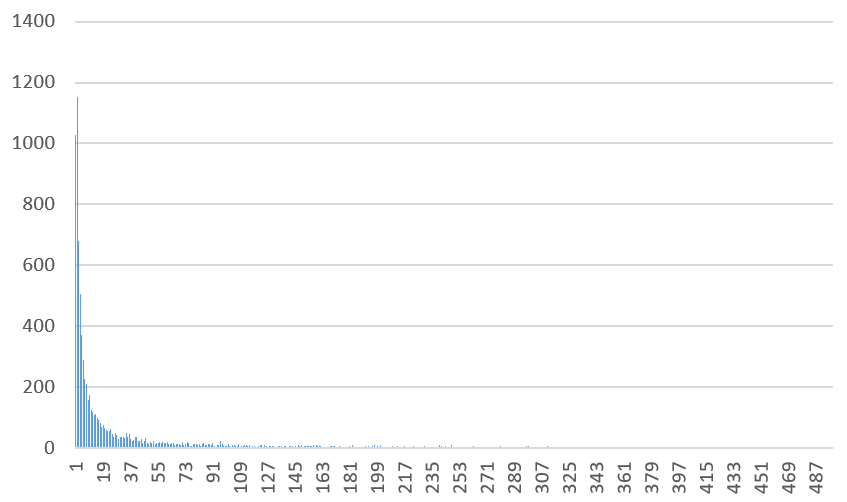
\includegraphics[width=0.7\textwidth]{figures/images/numberGenerator/powerlaw_-1_25.png}\label{fig:powerDistExample2}
\end{figure}
\subsection{RLS Comparison}
\makebox[\linewidth]{
\begin{tabular}{lp{3cm}p{6cm}p{6cm}}
\begin{tabular}[h]{cccccccc}
algo type&            \RLSN&     \RLSR&     \RLSR&     \RLSN&     \RLSR&     \RLSN&       RLS\\
algo param&             b=2&       s=3&       s=4&       b=3&       s=2&       b=4&         -\\
avg mut/change&       2.000&     1.996&     2.476&     3.000&     1.502&     4.000&     1.000\\
avg mut/step&         2.000&     2.000&     2.500&     3.000&     1.500&     4.000&     1.000\\
\hline
total avg count&     83,118&   104,748&   105,513&   112,223&   114,486&   121,927& 2,443,567\\
avg eval count&      83,118&   104,748&   105,513&   112,223&   114,486&   121,927&    45,834\\
max eval count&     778,110& 1,453,252&   898,974& 1,377,471&   915,268&   816,633&   485,275\\
min eval count&         197&       126&        45&       212&       271&       155&       128\\
\hline
fail ratio&           0.000&     0.000&     0.000&     0.000&     0.000&     0.000&     0.447\\
avg fail dif&             -&         -&         -&         -&         -&         -&         1\\
\end{tabular}
\end{tabular}
}


The input is even easier to solve for the RLS variants than the binomial distributed inputs.
There is no clear tendency and all algorithms have a rather equal runtime and also every algorithm manages to find an optimal solution in every run.
\subsection{(1+1) EA Comparison}
The first table shows the results for parameter $\beta=2.75$

\makebox[\linewidth]{
\begin{tabular}{lp{3cm}p{6cm}p{6cm}}
\begin{tabular}[h]{m{2.5cm}m{0,45cm}m{0,45cm}m{0,45cm}m{0,45cm}m{0,45cm}m{0,45cm}m{0,45cm}m{0,45cm}m{0,45cm}m{0,45cm}m{0,45cm}m{0,45cm}m{0,45cm}m{0,45cm}m{0,45cm}m{0,45cm}}
\multicolumn{1}{c}{algo type}&\multicolumn{2}{c}{           EA-SM}&\multicolumn{2}{c}{    EA-SM}&\multicolumn{2}{c}{    EA-SM}&\multicolumn{2}{c}{    EA-SM}&\multicolumn{2}{c}{    EA-SM}&\multicolumn{2}{c}{    EA-SM}&\multicolumn{2}{c}{    EA-SM}&\multicolumn{2}{c}{       EA}\\
\multicolumn{1}{c}{algo param}&\multicolumn{2}{c}{           50$/n$}&\multicolumn{2}{c}{    100$/n$}&\multicolumn{2}{c}{     10$/n$}&\multicolumn{2}{c}{      5$/n$}&\multicolumn{2}{c}{      4$/n$}&\multicolumn{2}{c}{      3$/n$}&\multicolumn{2}{c}{      2$/n$}&\multicolumn{2}{c}{        -}\\
\multicolumn{1}{c}{avg mut/change}&\multicolumn{2}{c}{     49.922}&\multicolumn{2}{c}{   99.873}&\multicolumn{2}{c}{   10.009}&\multicolumn{2}{c}{    5.053}&\multicolumn{2}{c}{    4.105}&\multicolumn{2}{c}{    3.156}&\multicolumn{2}{c}{    2.280}&\multicolumn{2}{c}{    1.534}\\
\multicolumn{1}{c}{avg mut/step}&\multicolumn{2}{c}{       49.989}&\multicolumn{2}{c}{  100.017}&\multicolumn{2}{c}{    9.999}&\multicolumn{2}{c}{    4.999}&\multicolumn{2}{c}{    4.005}&\multicolumn{2}{c}{    3.003}&\multicolumn{2}{c}{    2.000}&\multicolumn{2}{c}{    0.999}\\
\hline
\multicolumn{1}{c}{avg eval count}&\multicolumn{2}{c}{         84}&\multicolumn{2}{c}{      103}&\multicolumn{2}{c}{      111}&\multicolumn{2}{c}{      157}&\multicolumn{2}{c}{      184}&\multicolumn{2}{c}{      208}&\multicolumn{2}{c}{      273}&\multicolumn{2}{c}{      461}\\
\multicolumn{1}{c}{max eval count}&\multicolumn{2}{c}{      1,281}&\multicolumn{2}{c}{    1,488}&\multicolumn{2}{c}{    1,946}&\multicolumn{2}{c}{    3,030}&\multicolumn{2}{c}{    3,043}&\multicolumn{2}{c}{    3,283}&\multicolumn{2}{c}{    4,744}&\multicolumn{2}{c}{    7,036}\\
\multicolumn{1}{c}{min eval count}&\multicolumn{2}{c}{          0}&\multicolumn{2}{c}{        1}&\multicolumn{2}{c}{        3}&\multicolumn{2}{c}{        1}&\multicolumn{2}{c}{        0}&\multicolumn{2}{c}{        0}&\multicolumn{2}{c}{        2}&\multicolumn{2}{c}{        0}\\
\hline
\multicolumn{1}{c}{fail ratio}&\multicolumn{2}{c}{          0.000}&\multicolumn{2}{c}{    0.000}&\multicolumn{2}{c}{    0.000}&\multicolumn{2}{c}{    0.000}&\multicolumn{2}{c}{    0.000}&\multicolumn{2}{c}{    0.000}&\multicolumn{2}{c}{    0.000}&\multicolumn{2}{c}{    0.000}\\
&&&&&&&&&&&&&&&&\end{tabular}
\end{tabular}
}


Here the same rule holds for the RLS to some extent.
Until $p_m\le50/n$ the speed of convergence increases but at $p_m=100/n$ the speed decreases again.
The optimal value seems to be somewhere around $p_m=50/n$.
The (1+1) variants are generally faster than all RLS variants when comparing the maximum number of iterations.
For mutation rates $3/n\le p_m \le 100/n$ the (1+1) EA is also faster on average.
The next table shows the results for a powerlaw distribution with $\beta=1.25$.

\makebox[\linewidth]{
\begin{tabular}{lp{3cm}p{6cm}p{6cm}}
\begin{tabular}[h]{ccccccccc}
algo type&          (1+1) EA&   (1+1) EA&   (1+1) EA&   (1+1) EA&      (1+1) EA&   (1+1) EA&   (1+1) EA&   (1+1) EA\\
algo param&           3/n&     4/n&     2/n&     5/n&       -&    10/n&    50/n&   100/n\\
avg mut/change&     3.101&   3.968&   2.343&   4.859&   1.698&   9.732&  49.544&  99.494\\
avg mut/step&       2.999&   4.003&   2.002&   4.999&   1.001&   9.998&  49.998&  99.997\\
\hline
total avg count&      646&     701&     706&     857&   1,123&   1,508&   8,175&  15,485\\
avg eval count&       646&     701&     706&     857&   1,123&   1,508&   8,175&  15,485\\
max eval count&     5,346&   5,692&   3,415&   5,572&   7,001&  12,112&  52,831& 145,269\\
min eval count&        23&       4&      30&       9&      23&      14&      27&      69\\
\hline
fails&                  0&       0&       0&       0&       0&       0&       0&       0\\
fail ratio&         0.000&   0.000&   0.000&   0.000&   0.000&   0.000&   0.000&   0.000\\
avg fail dif&           -&       -&       -&       -&       -&       -&       -&       -\\
\end{tabular}
\end{tabular}
}


With this setting the optimal value is shifted to somewhere around $p_m=4/n$.
The higher mutation rates perform drastically slower with $p_m=100/n$ being 500 times slower than the optimal value.
The speed of convergence is sometimes even to slow find an optimal solution in time $10\cdot n\ln(n)$.
\subsection{pmut Comparison}
For pmut the same holds as for the RLS.\
The more bits the algorithms flips on average the better the performance on average.
Surprisingly the performance in the worst runs behaves inverted.
The fewer bits the algorithm flips on average the more stable the search becomes.
This might be caused by the really large amount of bits flipped for the lower values.

\makebox[\linewidth]{
\scriptsize
\begin{tabular}{lp{3cm}p{6cm}p{6cm}}
\begin{tabular}[h]{m{2.5cm}m{0,40cm}m{0,40cm}m{0,40cm}m{0,40cm}m{0,40cm}m{0,40cm}m{0,40cm}m{0,40cm}m{0,40cm}m{0,40cm}m{0,40cm}m{0,40cm}m{0,40cm}m{0,40cm}m{0,40cm}m{0,40cm}m{0,40cm}m{0,40cm}}
\multicolumn{1}{c}{algo type}&\multicolumn{2}{c}{            pmut}&\multicolumn{2}{c}{     pmut}&\multicolumn{2}{c}{     pmut}&\multicolumn{2}{c}{     pmut}&\multicolumn{2}{c}{     pmut}&\multicolumn{2}{c}{     pmut}&\multicolumn{2}{c}{     pmut}&\multicolumn{2}{c}{     pmut}&\multicolumn{2}{c}{     pmut}\\
\multicolumn{1}{c}{algo param}&\multicolumn{2}{c}{           3.25}&\multicolumn{2}{c}{     3.00}&\multicolumn{2}{c}{     2.75}&\multicolumn{2}{c}{     2.50}&\multicolumn{2}{c}{     2.25}&\multicolumn{2}{c}{     2.00}&\multicolumn{2}{c}{     1.75}&\multicolumn{2}{c}{     1.50}&\multicolumn{2}{c}{     1.25}\\
\multicolumn{1}{c}{avg mut/change}&\multicolumn{2}{c}{      1.583}&\multicolumn{2}{c}{    1.737}&\multicolumn{2}{c}{    2.002}&\multicolumn{2}{c}{    2.423}&\multicolumn{2}{c}{    3.303}&\multicolumn{2}{c}{    5.830}&\multicolumn{2}{c}{   12.519}&\multicolumn{2}{c}{   30.910}&\multicolumn{2}{c}{   73.182}\\
\multicolumn{1}{c}{avg mut/step}&\multicolumn{2}{c}{        1.729}&\multicolumn{2}{c}{    1.934}&\multicolumn{2}{c}{    2.274}&\multicolumn{2}{c}{    2.895}&\multicolumn{2}{c}{    4.360}&\multicolumn{2}{c}{    8.452}&\multicolumn{2}{c}{   22.278}&\multicolumn{2}{c}{   70.532}&\multicolumn{2}{c}{  224.421}\\
\hline
\multicolumn{1}{c}{avg eval count}&\multicolumn{2}{c}{        540}&\multicolumn{2}{c}{      569}&\multicolumn{2}{c}{      594}&\multicolumn{2}{c}{      641}&\multicolumn{2}{c}{      712}&\multicolumn{2}{c}{      808}&\multicolumn{2}{c}{      967}&\multicolumn{2}{c}{    1,285}&\multicolumn{2}{c}{    2,081}\\
\multicolumn{1}{c}{max eval count}&\multicolumn{2}{c}{      3,110}&\multicolumn{2}{c}{    2,891}&\multicolumn{2}{c}{    3,504}&\multicolumn{2}{c}{    3,896}&\multicolumn{2}{c}{    5,152}&\multicolumn{2}{c}{    4,274}&\multicolumn{2}{c}{    5,610}&\multicolumn{2}{c}{    6,190}&\multicolumn{2}{c}{   14,984}\\
\multicolumn{1}{c}{min eval count}&\multicolumn{2}{c}{         22}&\multicolumn{2}{c}{        9}&\multicolumn{2}{c}{       36}&\multicolumn{2}{c}{       25}&\multicolumn{2}{c}{       28}&\multicolumn{2}{c}{       27}&\multicolumn{2}{c}{       27}&\multicolumn{2}{c}{       13}&\multicolumn{2}{c}{       33}\\
\hline
\multicolumn{1}{c}{fail ratio}&\multicolumn{2}{c}{          0.000}&\multicolumn{2}{c}{    0.000}&\multicolumn{2}{c}{    0.000}&\multicolumn{2}{c}{    0.000}&\multicolumn{2}{c}{    0.000}&\multicolumn{2}{c}{    0.000}&\multicolumn{2}{c}{    0.000}&\multicolumn{2}{c}{    0.000}&\multicolumn{2}{c}{    0.000}\\
\hline
\multicolumn{1}{c}{p-value}&&\multicolumn{2}{c}{0.0000}&\multicolumn{2}{c}{0.0000}&\multicolumn{2}{c}{0.0000}&\multicolumn{2}{c}{0.0000}&\multicolumn{2}{c}{0.0000}&\multicolumn{2}{c}{0.0000}&\multicolumn{2}{c}{0.0000}&\multicolumn{2}{c}{0.0000}\\
&&&&&&&&&&&&&&&&&&\end{tabular}
\end{tabular}
}


The optimal value here seems to be somewhere around $\beta=1.5$, so only lightly smaller in comparison to the (1+1) EA where the optimal value almost change from one side of the spectrum to the other.
Here the inverted stability of the search does not occur.
The variants that take longer on average tend to also take longer in their worst runs.

\subsection{Comparison of the best variants}
The first table again shows the results for parameter $\beta=2.75$

\makebox[\linewidth]{
\begin{tabular}{lp{3cm}p{6cm}p{6cm}}
\begin{tabular}[h]{cccc}
algo type&            RLS&    pmut&      EA\\
algo param&             -&    3.25&       -\\
avg mut/change&     1.000&   1.287&   1.272\\
avg mut/step&       1.000&   1.729&   1.000\\
\hline
avg eval count&    91,171& 143,121& 231,082\\
max eval count&   153,143& 227,737& 446,942\\
min eval count&    65,783&  93,602& 165,818\\
\hline
fail ratio&         0.000&   0.000&   0.000\\
\end{tabular}
\end{tabular}
}


The ranking follows the amount of bits the algorithms flip on average per step.
$pmut_{1.25}$ manages to find the solution in just 56 iterations on average.
The (1+1) EA with $p_m=50/n$ is slower than $pmut_{1.25}$ but instead has a lower value for the maximum number of iterations.
Both options seem fine.
Even the \RLSN[4] is still very fast for the powerlaw distributed input with $\beta = 2.75$.
For $\beta = 1.25$ the results are a bit different.

The \RLSR[4] now performs equally good as the (1+1) EA variant with $p_m=4/n$, but is still slower than $pmut_{1.5}$.
As the first inputs were less difficult to solve than the inputs with $\beta = 1.25$ the second value was chosen for the evaluation of smaller input sizes.

\begin{tabular}[h]{ccccccccc}
fails in 1000 runs&20&50&100&500&1000&5000&10000&50000\\\hline
RLS&984&773&411&1&0&0&0&0\\
\RLSR[2]&890&241&14&0&0&0&0&0\\
(1+1) EA (1$/n$)&711&75&5&0&0&0&0&0\\
(1+1) EA (2$/n$)&541&14&0&0&0&0&0&0\\
pmut (3.0)&566&63&4&0&0&0&0&0\\
pmut (3.25)&587&63&7&0&0&0&0&0\\
\end{tabular}


The RLS is once again the algorithm that is the most likely to be stuck in a local optimum.
Compared to the other algorithms it is not as drastic as for the binomial input for example.
Only for $n<500$ the algorithms do not find a global optimum in every run.
The setting of the parameter almost doesn't affect the amount of runs without an optimal result.
The main differences are between the different algorithms themselves.
This type of input is probably easy to solve if it has a perfect partition.
The two stopping conditions where a step limit and finding a perfect partition or a partition with difference of one between the two bin for uneven $n$.
So in 80\% of the runs the algorithms might have found an optimal solution, but the stopping conditions did not trigger as the solutions where not close to a perfect partition.

\begin{tabular}[h]{ccccccccc}
avg&20&50&100&500&1000&5000&10000&50000\\\hline
RLS&32&79&153&579&950&1859&1922&1797\\
\RLSR[2]&391&2124&5005&4218&3530&2362&2160&2229\\
(1+1) EA (1$/n$)&22471&18343&12834&8342&6511&3815&3458&3371\\
(1+1) EA (2$/n$)&16360&9243&6452&4503&4020&3171&3141&3133\\
pmut (3.25)&23440&15929&9658&5644&4406&2434&2162&2172\\
pmut (3.0)&21901&14696&9186&5222&4150&2510&2208&2213\\
\end{tabular}


Looking at the time the algorithms needed on average the runs that hit the step limit could have possibly been no failed runs.
The easiest are inputs with size $n=500$.
For smaller values of $n$ the algorithms sometimes fail and even in a good run they need more iterations to find an optimal solution.
Due to the increasing size of the input the algorithms need more time for the bigger values.

\begin{tabular}[h]{ccccccccc}
total avg&20&50&100&500&1000&5000&10000&50000\\\hline
RLS&99470&93459&74385&3474&447&389&421&555\\
\RLSR[2]&96305&63088&19364&815&589&565&595&699\\
(1+1) EA (1$/n$)&89444&52886&21141&1410&869&850&875&1046\\
(1+1) EA (2$/n$)&79603&37214&14107&1302&992&942&957&1055\\
pmut (3.25)&84226&48403&18280&930&542&526&546&642\\
pmut (3.0)&82474&46286&17825&917&576&548&573&668\\
\end{tabular}



$pmut_{1.75}$ is not only the best variant for the bigger values of n but also for smaller inputs as well.
It is the least likely to be stuck in a local optimum, and it is also the fastest if it reaches a global optimum.
